\documentclass[a4paper,12pt]{article}
\usepackage[notoc,noabs]{HaotianReport}

\title{微信公众号数据可视化}
\author{刘昊天}
\authorinfo{队友:顾玥,黄凯欣}
\runninghead{清华大学《数据可视化》2019春季学期}
\studytime{2019年6月}

\begin{document}
    \maketitle
    \section{项目背景}
    随着智能手机的不断普及,移动社交软件已经成为人们生活的重要组成部分,而微信作为目前腾讯旗下赶超 QQ 的社交软件,更是在前几年迎来爆发式增长.根据腾讯控股 [00700]2018年年报,截止至 2018 年 12 月 31,微信合并月活跃用户数达 10.98 亿,同比增长 11.0\%;同时, 2018 年腾讯的网络广告业务收入达 581 亿元,同比增长 44\%.在微信及腾讯广告业务的发展过程中,微信公众号功不可没,其已经成为了国内最大的内容提供平台之一.个人或企业用户可以在微信公众号上发布文章,通过微信的订阅服务定向推送给已订阅的用户,无论是宣传还是营收都有巨大的空间;已订阅用户则可以消费微信公众号的推送内容.由此可见,微信公众号已经并将在很长一段时间内继续扮演中国人生活中的重要角色.

    与此对应的,作为个人用户,我们对某一特定的微信公众号并没有方便的认知渠道.当我们看到某一个公众号,我们只能通过阅读简介或查看朋友关注数、历史文章数等方式对一个公众号进行直观的了解,并可能阅览有限的几篇历史文章进行进一步了解.这种程度的认知,并不足以为我们判断其内容质量、权威性、主题、同自身兴趣契合程度等提供充分的指导.因此,如果能对微信公众号的数据进行分析与可视化,将该公众号的内容简洁、直观、充分地呈现给用户,则将在精准内容选择方面提供巨大的帮助.

    2019 年 3 月 31 日,咪蒙发布朋友圈调侃“第二次开垮公司”,宣告其旗下的北京〸月初五影视公司正式解散;而就在 2018 年底,咪蒙公开数据称其公众号"1400 万粉丝,单篇最高阅读量为 1470 万".朋友圈中,一度出现了" 含咪率"(个人朋友中关注咪蒙公众号的比例)这样调侃的词汇.可见公众号对舆论影响之重大,更凸显了对公众号分析的必要性.

    综上,本任务拟通过对微信公众号相关数据的分析与可视化,体现特定公众号的内容质量、权威性、主题,展现某些公众号间的关联,促进用户对内容的精准选择.
    \section{可视化设计与实现}
    \subsection{完成情况}
    经过分析,本可视化任务可以被分为四个方面,即:
    \begin{enumerate}
      \item 公众号自身指标的评价;
      \item 公众号之间的对比、关联;
      \item 推送文章自身的评价;
      \item 推送文章之间的对比、关联。
    \end{enumerate}

    鉴于时间安排和工作能力的考虑,我们完成了上述任务中的1、3、4三个方面,第2个方面没有涉及,是本项目的一个遗憾。项目制定的总体计划如\cref{fig:taskmindmap}所示。
    \begin{figure}
      \centering
      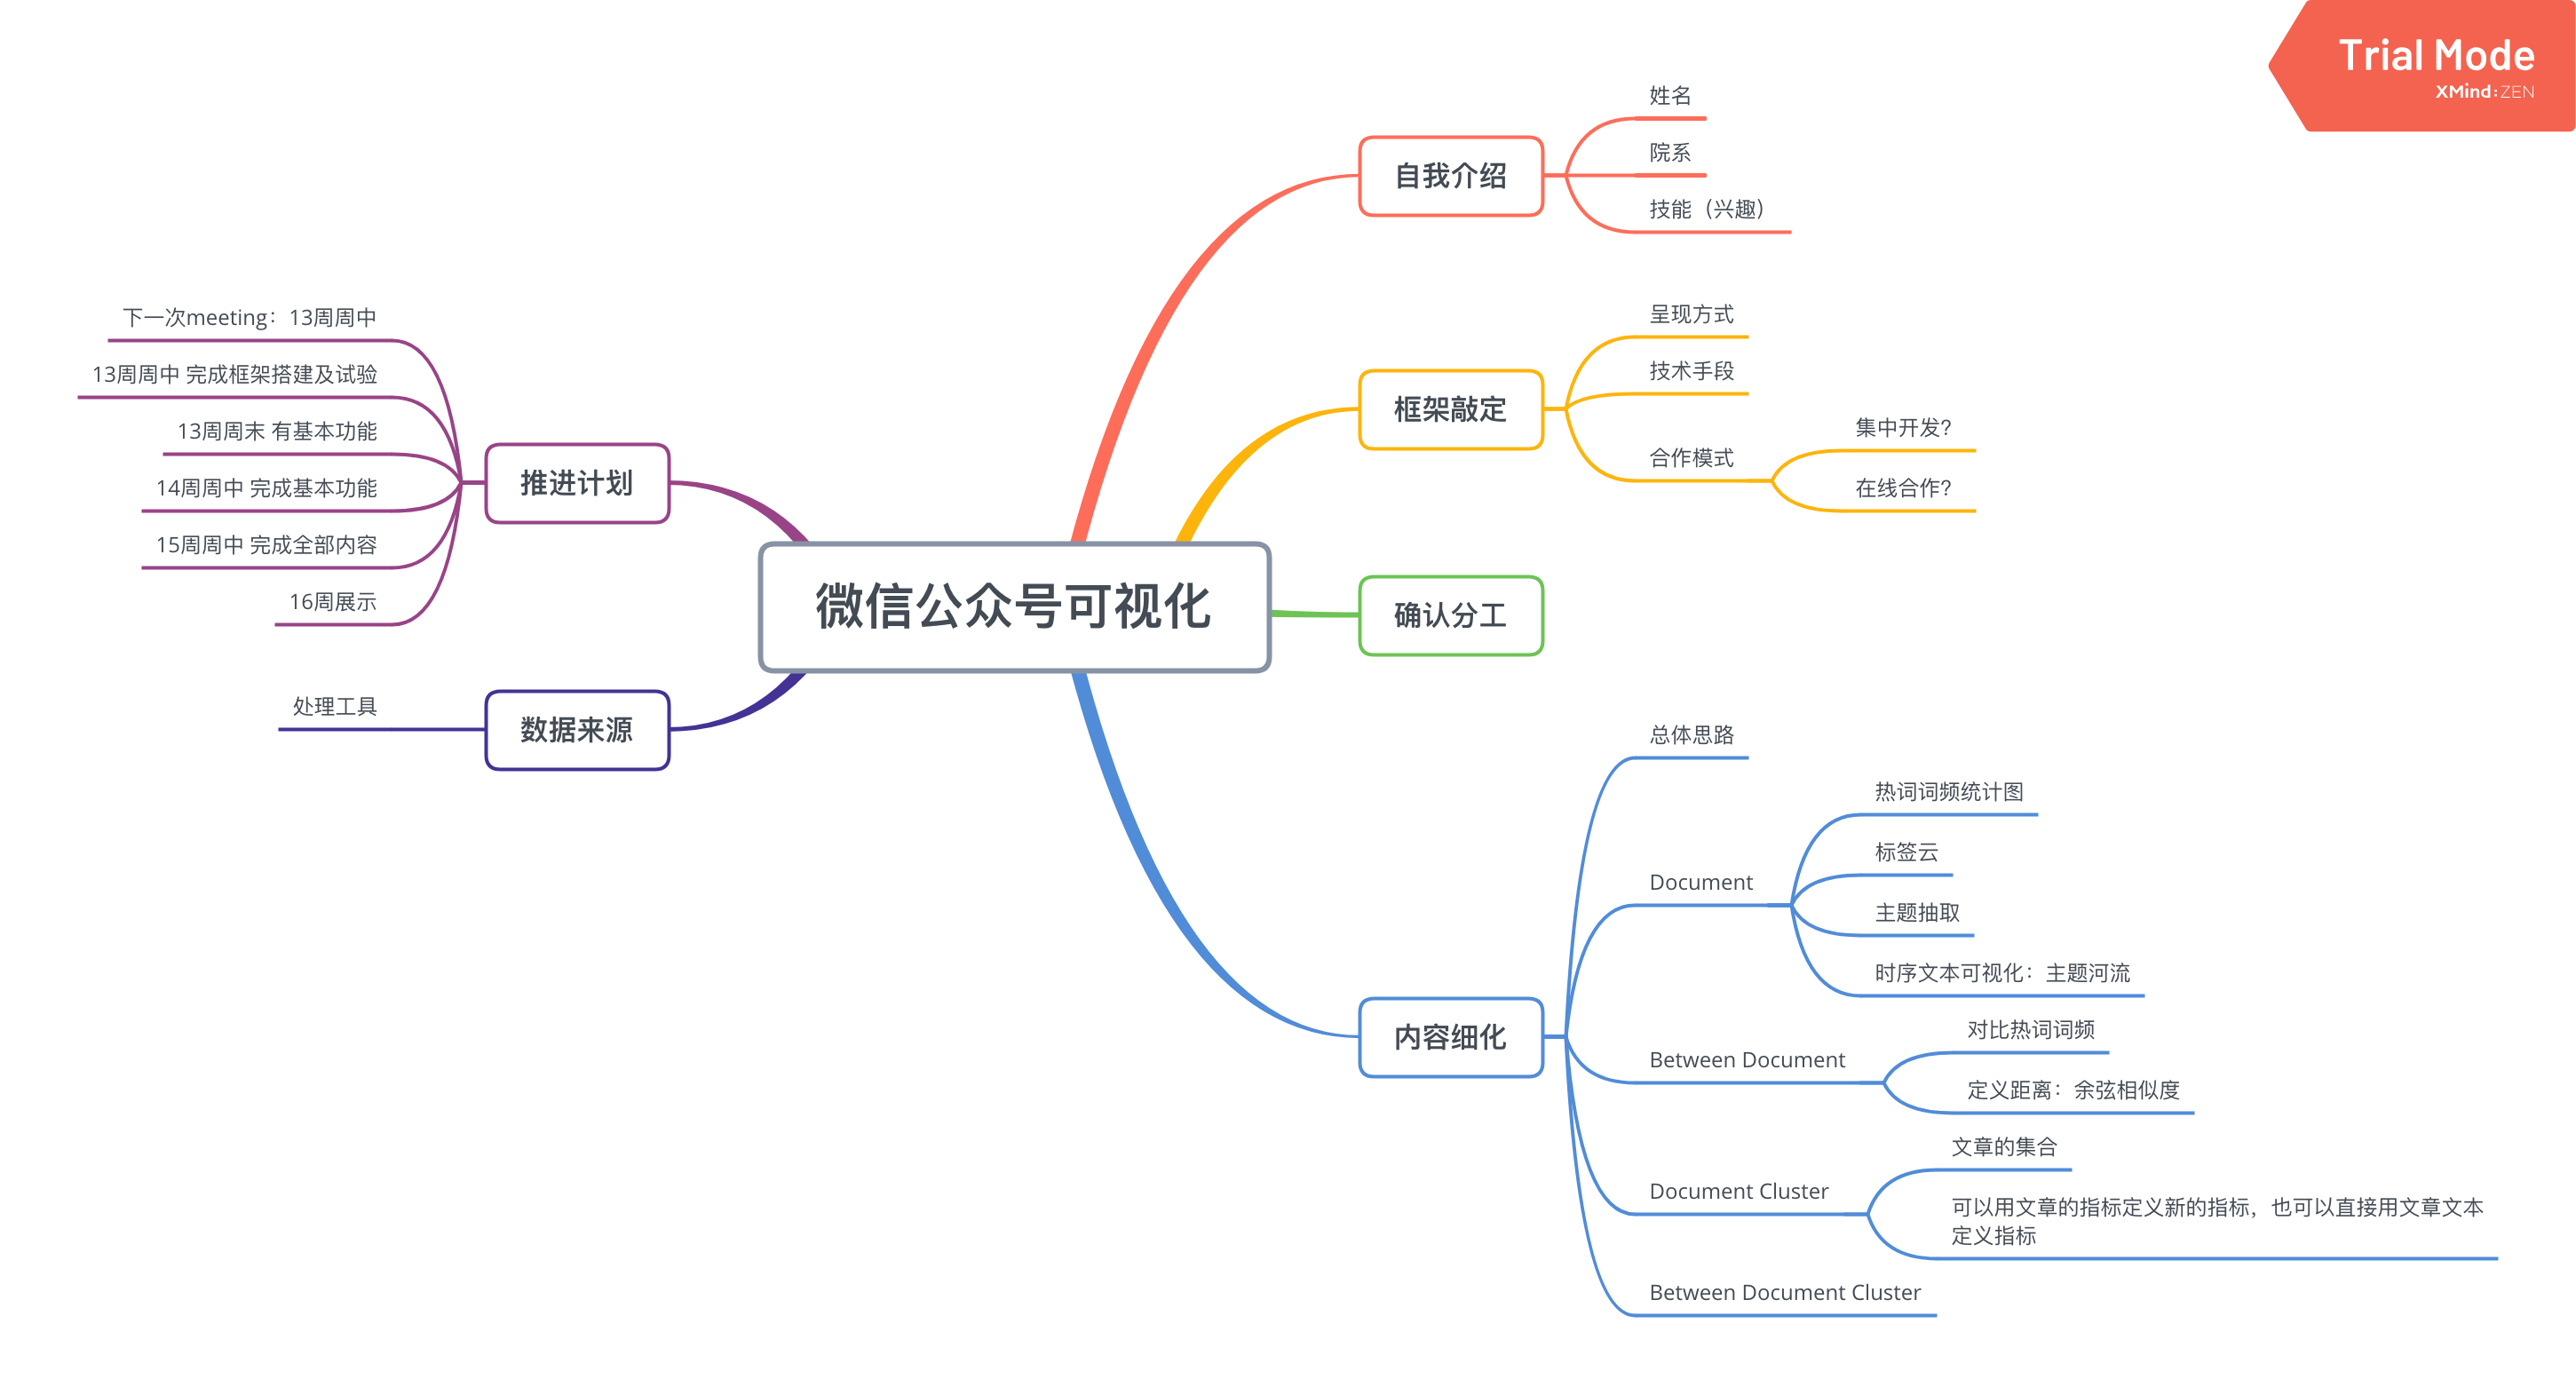
\includegraphics[width=0.95\linewidth]{TasksMindmap.png}
      \caption{思维导图}
      \label{fig:taskmindmap}
    \end{figure}
    \subsection{项目框架}
    作为一个完整的可视化任务,我们不能简单地将各个子任务拼接在一起,而是应该将其组织为一个有机的整体。为了实现这个目标,我们设计了一套前后端分离的系统架构。其中,前端设计为一个页内APP,从后端拉取数据后进行可视化绘制;后端作为一个数据提供接口,在爬取数据后进行处理,并通过api将数据提供给前端。简单来说,项目框架的大致情况如下:
    \begin{enumerate}
      \item 代码托管:Github:ritou11/wxPubVis
      \item 可视化工具:D3.js
      \item NLP工具:snowNLP.py, jieba.py
      \item API标准:GraphQL
      \item 前端框架:React+Redux
      \item 部署:Docker工具链
      \item CI/CD:Shippable/Netlify
      \item 视觉:Material UI
      \item 其他:借用了Bootstrap样式库中的部分样式
    \end{enumerate}
    \subsection{公众号自身指标评价}
    \subsubsection{散点图:推送分布}
    采用散点图的形式,展现公众号推送随时间的分布情况。其中,横轴为推送发表时间,纵轴为阅读量。该分布可以展示公众号发表推送的火热程度,一定程度反映内容质量。同时,为了在视觉中编码更多信息,我们采用颜色通道,特别是HSL空间中的S和L通道,编码推送的读者情感色彩。颜色越红越鲜艳,代表推送的读者情感色彩越积极正面。

    “推送的读者情感色彩”,是通过每篇推送下方的读者留言计算的,采用了开源NLP库snowNLP。当然,部分推送没有留言,在图中呈现为灰白色。

    由于此部分订制程度不高,主要是设计,因此在实现时采用了强大的Highcharts.js可视化包。
    \begin{figure}
      \centering
      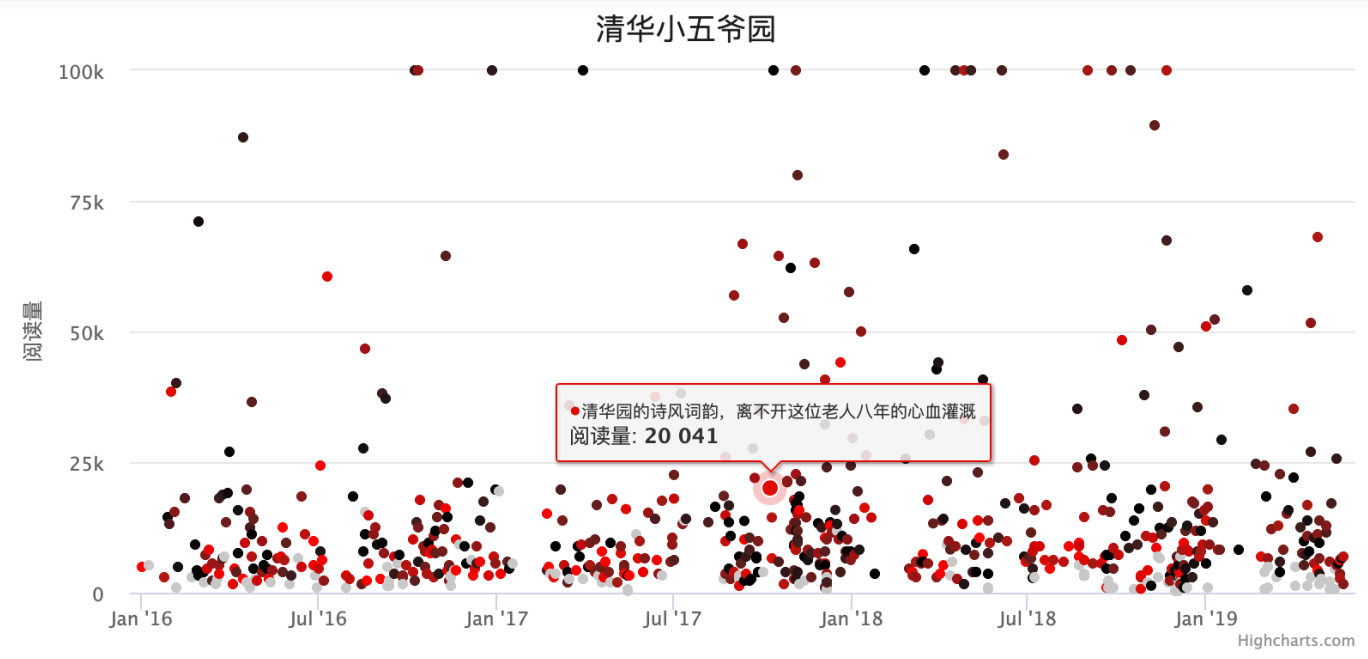
\includegraphics[width=0.95\linewidth]{sdt.png}
      \caption{散点图:推送分布}
      \label{fig:sdt}
    \end{figure}
    \subsubsection{折线图:活跃度}
    采用折线图的形式,展现公众号的活跃度随时间的变化情况。其中,横轴为时间,纵轴为公众号活跃度。

    活跃度的计算,是包含了该公众号当天发表推送的数量和质量(阅读数+点赞数)的,计算公式如下:
    \[
      H_i = \frac{\sum_{j\in{P_i}}(y_{ij}+50z_{ij})}{\sqrt{n_i}}
    \]
    其中$H_i$为第$i$天的活跃度,$P_i$为第i天的推送标号集合,$y_{ij}$代表第$i$天第$j$篇推送的阅读量,$z_{ij}$代表第$i$天第$j$篇推送的点赞数。

    \cref{fig:zxt}展现了公众号“洞见”的活跃度变化情况,从中可以看出,在18年末时,洞见开始爆发式增长,可以推断其在这个时间点改变了运营策略。

    由于此部分订制程度不高,主要是计算指标,因此在实现时采用了强大的Highcharts.js可视化包。
    \begin{figure}
      \centering
      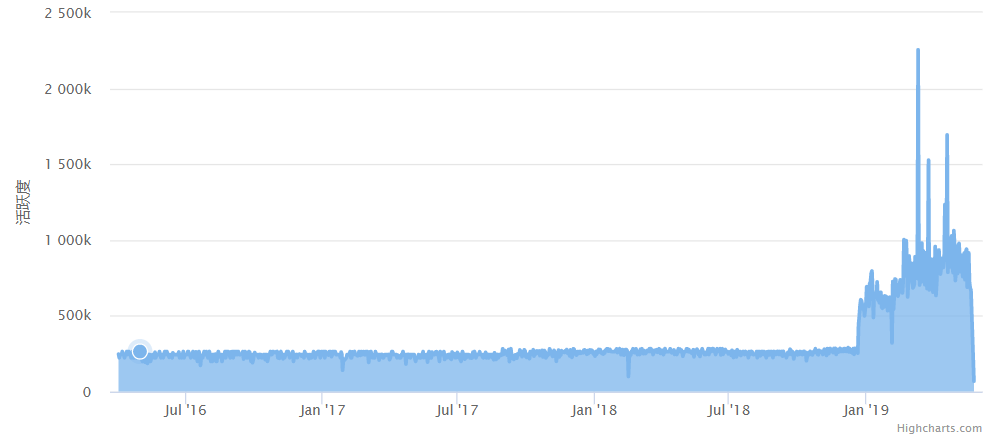
\includegraphics[width=0.95\linewidth]{zxt.png}
      \caption{散点图:推送分布}
      \label{fig:zxt}
    \end{figure}
    \subsubsection{树图:主题分布}
    树图展示了每个公众号的主体。每个公众号分别提取了30个主题,每个主题由一组词汇进行描述。在树图中,面积编码了主题的重要性占比,而在鼠标悬浮在对应的主题色块上时,浮动跟随的卡片中展示了该主题的内容。

    该部分实现应用了D3的内部工具,方法同第二次小作业相同。

    \begin{figure}
      \centering
      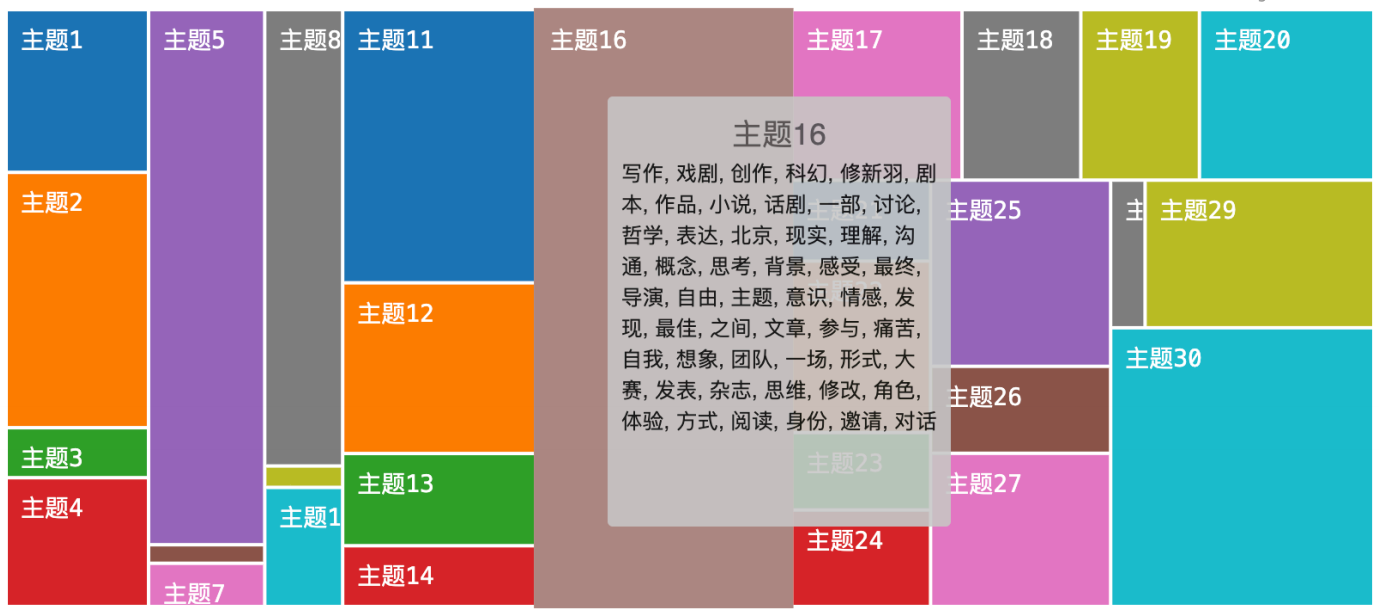
\includegraphics[width=0.95\linewidth]{st.png}
      \caption{树图:主题分布}
      \label{fig:st}
    \end{figure}
    \subsection{推送自身指标评价}
    \subsubsection{文档卡片:基本信息}
    文档卡片包含了一篇推送的关键信息,包括封面图、所属公众号、阅读量、点赞数、标题、简介、发表时间等等。

    \begin{figure}
      \centering
      
\includegraphics[width=0.3\linewidth]{wdkp.png}
      \caption{文档卡片:基本信息}
      \label{fig:wdkp}
    \end{figure}
    \subsubsection{“主题条”+词云:主题情况}
    “主题条”是本项目新的一个命名,这是一个占地面积很小的可视化结果,适合插入到各种页面中。其中,每个主题的宽度编码了主题的重要程度。将鼠标悬浮在对应的主题上时,浮动的卡片中展示了该主题包含的关键词词云。词云的字体大小编码了该关键词在主题中的重要程度。

    \begin{figure}
      \centering
      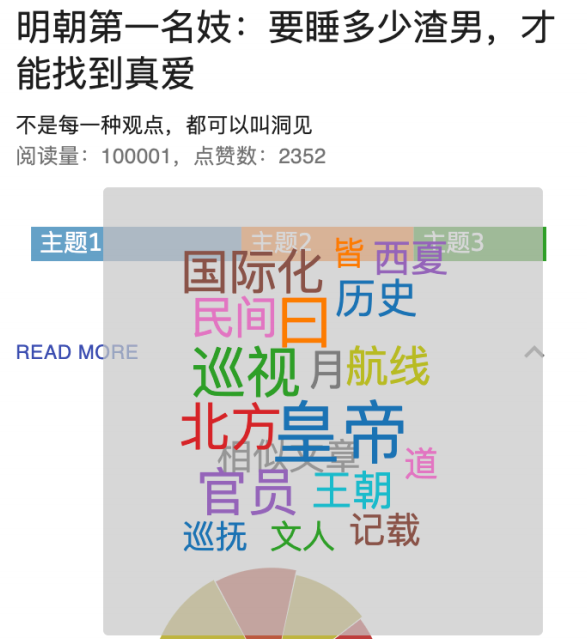
\includegraphics[width=0.5\linewidth]{ztt.png}
      \caption{“主题条”+词云:主题情况}
      \label{fig:ztt}
    \end{figure}
    \subsection{推送之间的对比关联}
    \subsubsection{玫瑰图:相似文章}
    使用玫瑰图作为相似文章的推荐,也是本项目的一个创新之处。玫瑰图每个花瓣的半径代表了相似度,角度代表了阅读量,颜色代表对应⽂文章的读者感情色彩,颜色越红感情越积极。鼠标悬浮在花瓣上,浮窗展示了推送标题;点击一个花瓣,可跳转到对应推送的可视化页面。

    相似度的计算使用的是余弦相似度,与授课讲解的一致,基于sklearn.metrics包。
    \begin{figure}
      \centering
      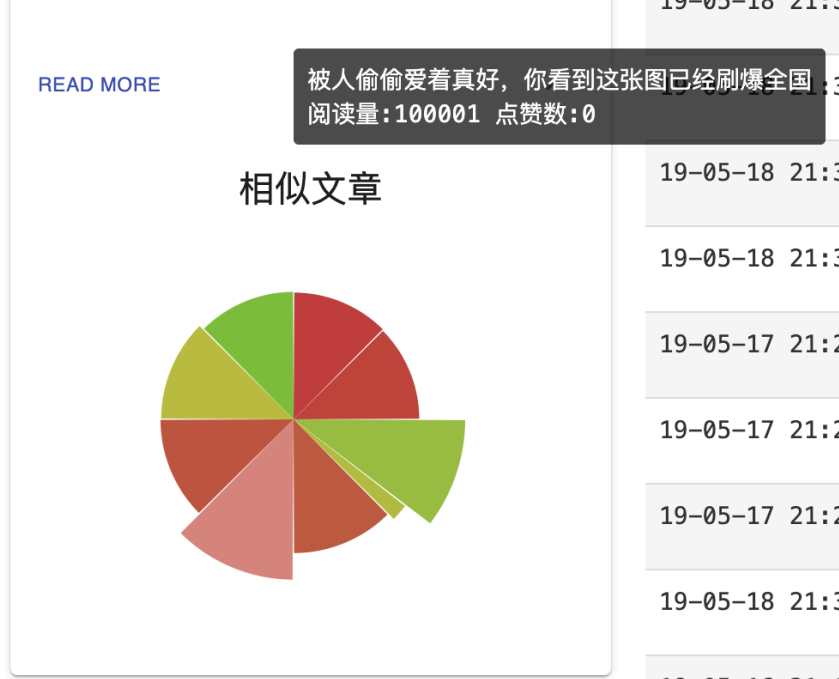
\includegraphics[width=0.5\linewidth]{mgt.png}
      \caption{玫瑰图:相似文章}
      \label{fig:mgt}
    \end{figure}
    \section{可视化系统案例分析}
    本项目体现的方式,是一个可以交互的网站平台。项目的访问地址为:\url{https://wxpub.nogeek.top},长期有效。

    此处展示两个主要页面,在上述可视化任务分析中并没有展示。其一为公众号页面,如\cref{fig:zym}所示。该页面左侧为公众号相关指标的可视化,可滚动切换查看;右侧为公众号列表,包含了公众号数据的爬取情况。点击详情按钮,可以切换到对应公众号的可视化图像。点击公众号名称,可以查看对应公众号的全部推送,跳转到推送页面。
    \begin{figure}
      \centering
      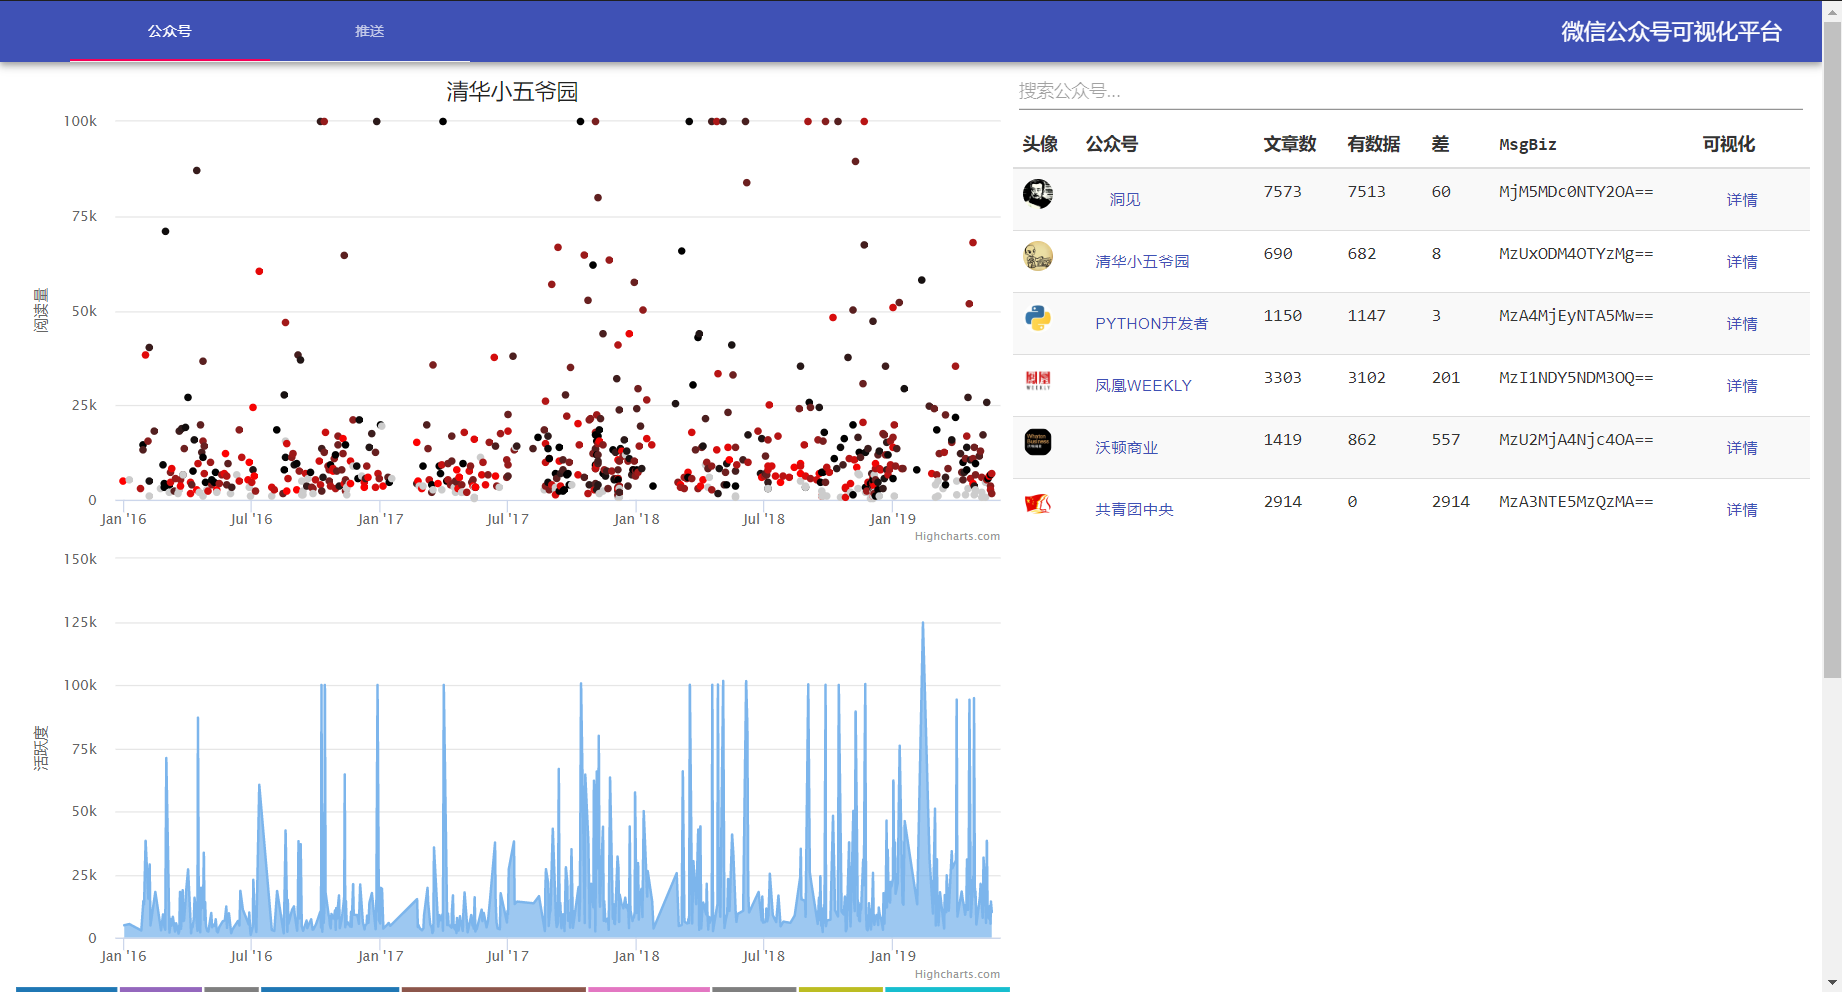
\includegraphics[width=0.9\linewidth]{zym.png}
      \caption{公众号页面}
      \label{fig:zym}
    \end{figure}

    推送页面如\cref{fig:tsym}所示。推送页面的左侧是一个文档卡片,展示了关于该推送的方方面面,点击卡片右下角的箭头,可以展开相关推送的推荐(玫瑰图)。页面右侧为推送列表,还包含了分页器和筛选器,可以方便地浏览、查询、排序推送;列表的内容为推送的基本信息,点击详情按钮可以在文档卡片中查看对应推送;点击推送标题,可以跳转到对应推送的原始链接;点击公众号,可以跳转回对应公众号的可视化页面。
    \begin{figure}
      \centering
      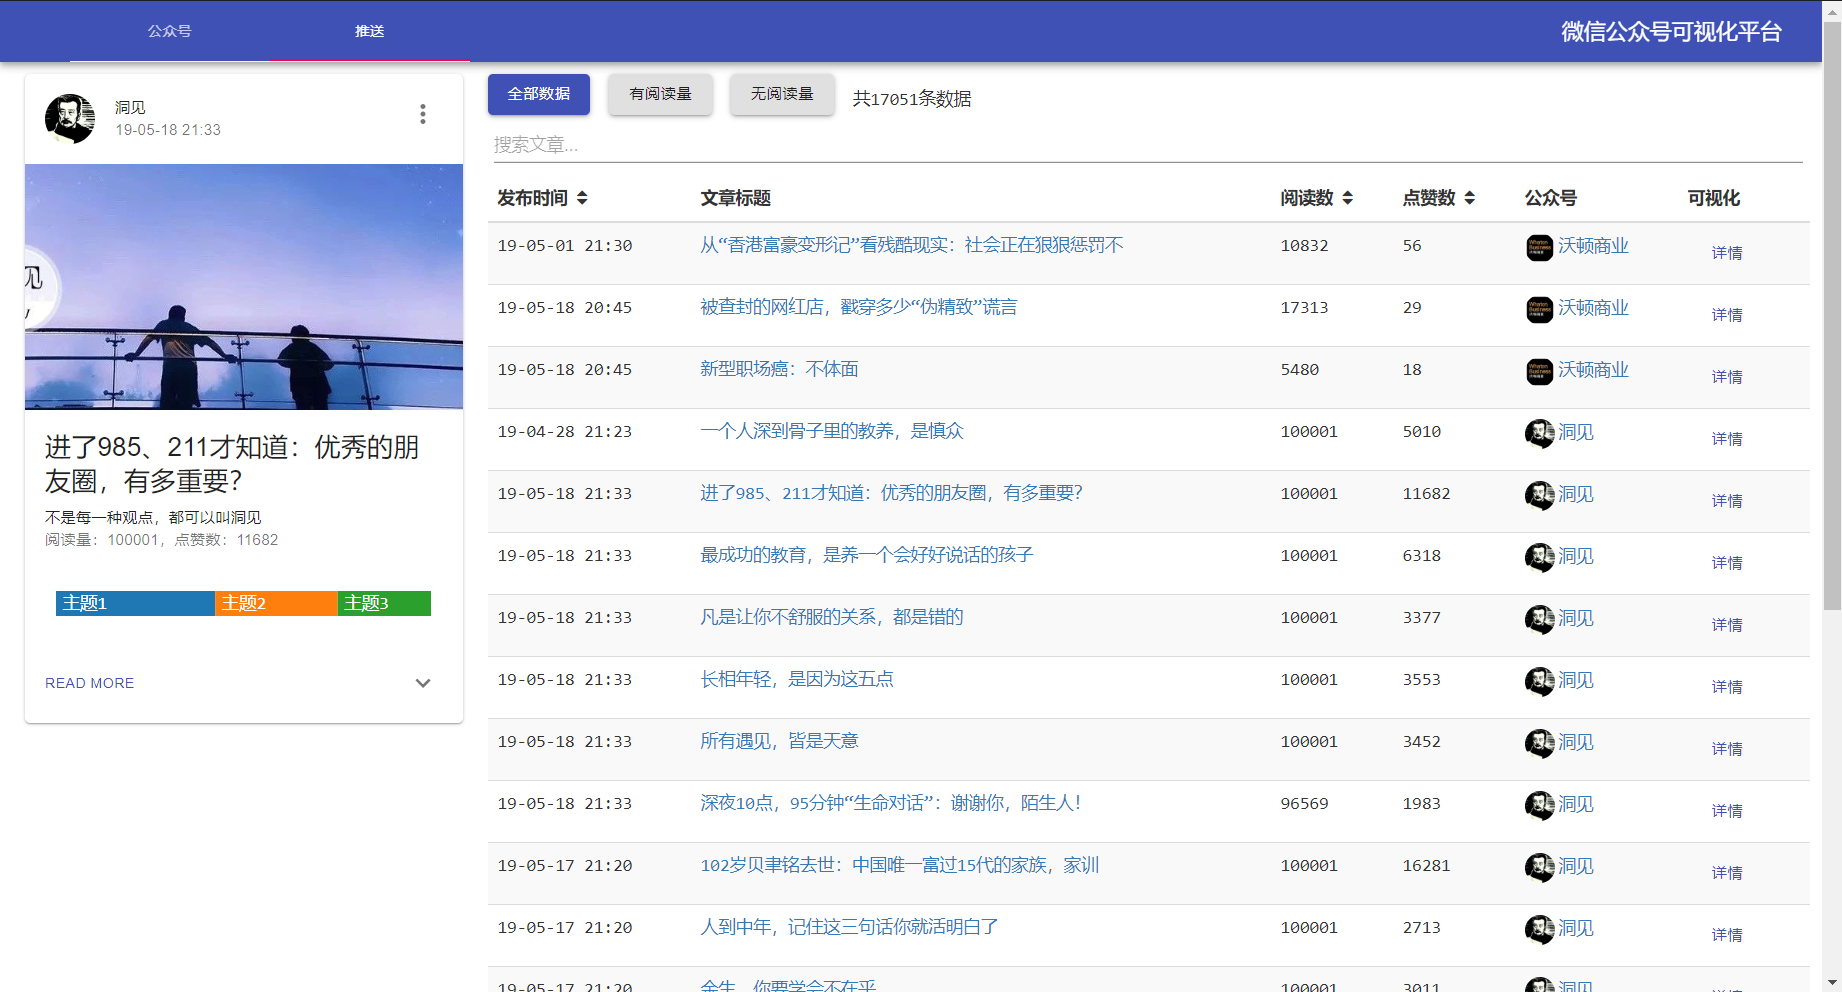
\includegraphics[width=0.9\linewidth]{tsym.png}
      \caption{推送页面}
      \label{fig:tsym}
    \end{figure}
    \label{applastpage}

    更为详尽的Step-By-Step的介绍,在提交的视频中已经涉及,在此不再赘述。
    \section{项目分工}
    本项目本有四名成员:刘昊天、顾玥、黄凯欣、于丹阳,但于丹阳同学在第一次项目讨论会后,便未曾参与项目的任何推进;在最后的文档制作中,本应其完成的PPT和报告,皆由刘昊天在多次联系不上后,紧急完成。

    项目分工如下:
    \begin{enumerate}
      \item 刘昊天:完成大部分的项目开发工作,工作量60\%。
      \item 顾玥:完成文本数据的处理与计算,工作量30\%。
      \item 黄凯欣:完成少量可视化任务,并参与多次讨论,工作量10\%。
    \end{enumerate}
    % \newpage
    % \bibliography{report}
    % \bibliographystyle{unsrt}
\iffalse
\begin{itemize}[noitemsep,topsep=0pt]
%no white space
\end{itemize}
\begin{enumerate}[label=\Roman{*}.,noitemsep,topsep=0pt]
%use upper case roman
\end{enumerate}
\begin{multicols}{2}
%two columns
\end{multicols}
\fi
\end{document}
